\section{\texorpdfstring{Silne regularni grafy, propletani vl cisel}{Silne regularni grafy, propletani vl cisel}}
\vspace{5mm}
\large

\begin{definition}
	Silne regularni je graf pokud neni uplny (trivialni pripad) a $\exists d,e,f \in \N: \forall v \in V \ deg(v) = d$.
	Kazde 2 sousedni vrcholy maji e spolecnych sousedu (2 vrcholy lezi v e $\triangle$), kazde 2 nesousedni vrcholy maji f spolecnych sousedu ($\exists f$ cest delky 2).
\end{definition}

\begin{theorem}[Silne regularni grafy (nebude u zkousky)]
	Je-li G silne regularni s parametry $d,e,f$, pak nastava jedna z 2 moznosti:
	\begin{itemize}
		\item $f = e + 1, d = 2f, |V(G)| = 2d + 1$ nebo
		\item $\exists s \in \N: s^2 = (e - f)^2 - 4(f - d) \land \frac{d}{2fs}((d - 1 + f - e)(s + f - e) - 2f) \in \N$.
	\end{itemize}
\end{theorem}
\begin{proof}
	Necht A je matice sousednosti G, $n = |V(G)|$, uvazme $A^2$.
	Na diagonale jsou stupne $d$, mimo diagonalu pokud v A byla 1 - zmeni se na e, 0 se zmeni na f.

	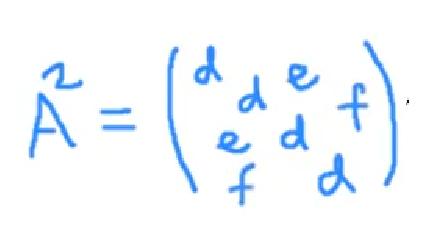
\includegraphics[scale=0.5]{s_reg_1.eps}

	\[ A^2 = dI + eA + (J -I - A)f \Rightarrow A^2 + (f - e)A + (f - d)I = fJ \]
	Dosadime vl. cislo $\lambda \in Sp(A)$.
	\[ \lambda^2 + (f - e)\lambda + (f - d) \in Sp(fJ) = \{ f * n, 0^{(n-1)} \} \]

	d odpovida vl. vektoru $\bar{1}$ u A, u J vl. vektoru $\bar{1}$ odpovida n. Dosadime d:
	\[ d^2 + (f - e)d + f - d = fn \Rightarrow d(d - e - 1) = f(n - d - 1)\]

	Zafixujme nejaky vrchol $x \in V$. Kolik $\exists$ indukovanych cest delky 2:
	\[ |\{ (x,a) | xa, ab \in E(G) \land xb \notin E(g) \}| \]

	Mame d zpusobu zvolit souseda x, pak vrchol a ma d sousedu, e jsou spolecne s x, x taky patri mezi sousedy. Dostaneme $d (d - e - 1)$.
	Na druhou stranu z pohledu vrcholu b. X ma $(n - d - 1)$ nesousedu, pak vrchol a je mezi f sousedu $(x,b)$. Dostaneme $f(n - d - 1)$.

	Pro $\lambda \in Sp(A)\setminus \{d\}$ zbyva 0:
	\[ \lambda^2 + (f - e)\lambda + f - d = 0 \Rightarrow \lambda_{1,2} = \frac{e - f \pm \sqrt{(e - f)^2 - 4 (f - d)}}{2} \]
	Oznacme $D = \sqrt{(e - f)^2 - 4 (f - d)}$. Pak $\lambda_1 = 1/2 (e - f + s), p$ krat a $\lambda_2 = 1/2 (e - f - s), q$ krat.

	Z nasobnosti vl. cisel
	\begin{equation*}
	\begin{aligned}
	 1 + p + q = n \\
	 a + p\lambda_1 + q \lambda_2 = tr(A) = 0 \\
	 tr(A^2) = \sum \lambda_i^2 = nd \Rightarrow d^2 + p \lambda_1^2 + q \lambda_2^2 = nd
	\end{aligned}
	\end{equation*}

	Vyresime soustavu 3 rovnic o 3 neznamych.
	Dosadime hodnoty $\lambda_1, \lambda_2$ do 2. rovnici:
	\[ d + 1/2 p (e - d + s) + 1/2 q (e - f - s) = 0 \Rightarrow d + 1/2(p + q) (e - f) + 1/2 (p - q) s = 0 \]

	Nastavaji 2 pripady:\\
	1) $s \notin \Q \Rightarrow$ posledni scitanec je iracionalni a nutne $ p = q = 1/2 (n - 1)$.
	\[ d + 1/2 (n-1) (e - f) = 0 \Rightarrow \frac{2d}{n - 1} = (f - e) \]
	Pak stupen vrcholu $ d \leq (n - 1)$
	\[ \frac{2d}{n - 1} = (f - e) \leq \frac{2 (n-1)}{2} = 2 \]
	Pokud $(f - e) = 2 \Rightarrow d = n-1 \Rightarrow G = K_n$ coz jsme vyloucili definici. Jinak
	\[(f - e) = 1 \land n = 2d + 1 \]
	Pracujme s 3. rovnici:
	\[ d^2 + 1/2 (n-1) * 1/4 (e - f + s)^2 + 1/2 (n-1) * 1/4 (e - f -s)^2 = nd \]
	dosadime $(e - f) = -1$.
	\begin{equation*}
	\begin{aligned}
	 d^2 + 1/2 (n-1) * 1/4 (s - 1)^2 + 1/2 (n-1) * 1/4 (-1 - s)^2 = nd \\
	 8d^2 + (n-1)(s^2 - 2s + 1) + (n-1)(s^2 + 2s + 1) = 8nd \\
	 8d^2 + (n-1)(s^2 - 2s + 1 + s^2 + 2s + 1) = 8nd \\
	 8d^2 + (n-1)(2s^2 + 2) = 8nd \\
	 4d^2 + (n-1)(s^2 + 1) = 4nd
	\end{aligned}
	\end{equation*}
	Dosadime $n = 2d - 1$
	\[ 4d^2 + 2d(s^2 + 1) = 4(2d + 1)d \]
	\[ 2d + (s^2 + 1) = 2(2d + 1) \]
	Pak $s^2 = 1 + 4(d - f)$
	\[ 2d + 2 + 4d - 4f = 4d + 2 \]
	\[ 2d = 4f \Rightarrow d = 2f \]
	2) Jinak $s \in \Z$ Dosadime do 2. a 3. rovnice n, vyresime pro p,q.
	\begin{equation*}
	\begin{aligned}
		d + 1/2 p (e - d + s) + 1/2 q (e - f - s) = 0 \\
		d^2 + 1/2 (n-1) * 1/4 (e - f + s)^2 + 1/2 (n-1) * 1/4 (e - f -s)^2 = (1 + q + p)d \\
	\end{aligned}
	\end{equation*}
	Zbavime se jmenovatele a roznasobime kvadraty v 3.
	\begin{equation*}
	\begin{aligned}
		p (e - d + s) + 1/2 q (e - f - s) = 2d \\
		p((e - f + s)^2 - 4d) + q((e - f -s)^2 - 4d) = 4d (1 - d)
	\end{aligned}
	\end{equation*}
	Spocitame p,q pomoci determinantu.

	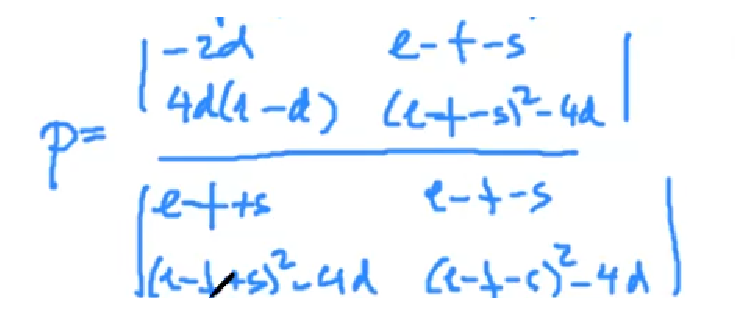
\includegraphics[scale=0.5]{s_reg_2.eps}

	Dolni determinant
	\begin{equation*}
	\begin{split}
		(e - f + s)((e - f - s)^2 -4d) - (e - f - s)((e - f + s)^2 - 4d) = \\
		(e - f + s)(e - f - s)(e - f -s - e + f - s) + 4d (e + f - s + e - f - s) = \\
		((e - f)^2 - s^2)(-2s) + 4d (-2s) = (-2s)((e - f)^2 + 4d - s^2)
	\end{split}
	\end{equation*}
	Dosadime $s^2 = (e - f)^2 + 4(d - f)$.
	\[ (-2s)((e - f)^2 + 4d - (e - f)^2 + 4(d - f)) = -8fs \]

	Horni determinant:

	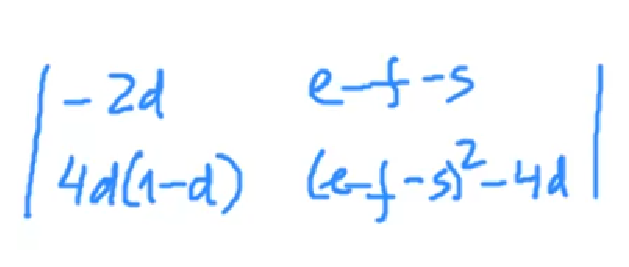
\includegraphics[scale=0.5]{s_reg_3.eps}

	2 houts later...
	\[ p = \frac{d((d - 1 + f - e)(s + f - e) - 2f)}{2fs} \in \Z \]
\end{proof}

\begin{theorem}[Friendship theorem]
	Necht v grafu G maji kazde 2 ruzne vrcholy prave 1 spol. souseda.
	Pak G obsahuje vrchol, ktery sousedi se vsemi ostatnimi vrcholy grafu.
\end{theorem}
\begin{proof}
	Pokud plati $ e = f = 1 \Rightarrow \exists v \in V$ ktery sousedi se vsemi ostatnimi vrchly. \\
	Necht $N_G(u)$ je mnozina sousedu $u \in V$. Vezmeme mnozinovy system $\{ N_G(u) | u \in V \}$.

	Pak prunik dvou mnozin je jednoprvkovy.
	\[ \forall a \ne b: |N_G(a) \cap N_G(b)| = 1 \]
	Taky z obrazku

	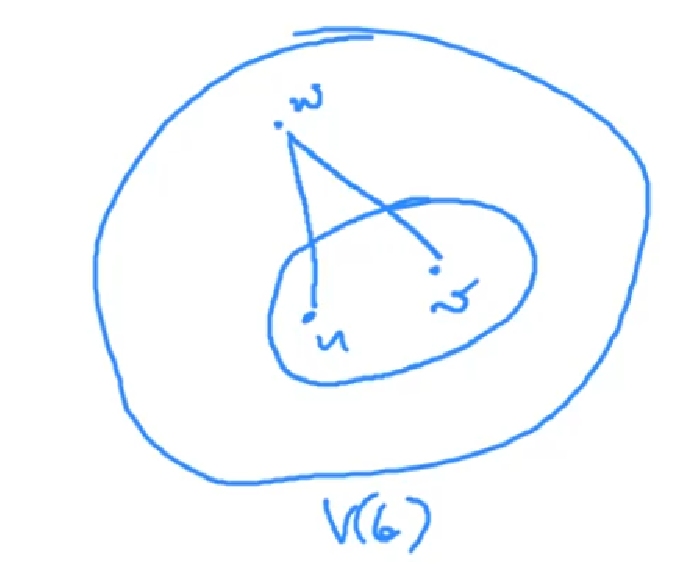
\includegraphics[scale=0.5]{fiendship_1.eps}

	\[ \forall a \ne b\ \exists! N_G(w): a,b \in N_G(w) \]
	Coz je skoro konecna projektivna rovina KPR. Chybi 3. axiom. Rozebereme 2 pripady:

	1) 3. axiom plati $\Rightarrow \{N_G\}$ je KPR. Pak
	\begin{equation*}
	\begin{split}
		\forall a |N_G(a)| = m + 1 = deg(a) \\
		n = |V(G)| = m^2 + m + 1\\
	\end{split}
	\end{equation*}
	Z cehoz G je silne regularni s parametry $ d = m + 1 \land e = f = 1$. Prvni pripad nastat nemuze kvuli podmince na $e = f = 1$. Neboli 2 pripad:

	\begin{equation*}
	\begin{aligned}
		p = \frac{d((d - 1 + f - e)(s + f - e) - 2f)}{2fs} \in \Z \\
		(e - f)^2 - 4 (f - d) = s^2 \land e = f = 1 \Rightarrow s = 2 \sqrt{m} = 2t
	\end{aligned}
	\end{equation*}
	Dosadime
	\[ p = \frac{t^2 + 1}{4t}((t^2 * 2t) - 2) = \frac{(t^2 + 1)(t^3 - 1)}{2t} \notin N : t > 1 \]
	Pripad $t = 1 \Rightarrow m = 1$ neni zajimavy protoze KPR radu 1 je $\triangle$.

	2) 3. axiom neplati $\Rightarrow \{N_G\}$ z teorie KPR bud vsechno lezi na 1 primce nebo jeden vrchol samostatne a zbytek na primce. Pak ten sampstatny vrchol je hledany soused vsech:
	\[ \exists a : N_G(a) = V(G)\setminus \{a\} \]

\end{proof}
\begin{theorem}[vl cisla Hermitovske matice]
	Necht $A \in \Comp^{n \times n}$ je Hermitovska, $\lambda_1 \geq \lambda_2 \geq ... \geq \lambda_n$ jeji vl. cisla.
	Necht $b_1, b_2, ..., b_n \in \Comp^n$ je ortonormalni baze vl vektoru. Pak pro $k = 1, 2, ..., n$ plati
	\[ x^{\ast}Ax \geq \lambda_k x^{\ast}x \forall x \in \langle \{ b_1, b_2, ..., b_k\} \rangle \]
	\[ x^{\ast}Ax \leq \lambda_k x^{\ast}x \forall x \in \langle \{ b_k, b_{k+1}, ..., b_n\} \rangle \]
\end{theorem}

\begin{theorem}[Propletani vl cisel]
	Necht $A \in \Comp^{n \times n}$ je Hermitovska, $\lambda_1 \geq \lambda_2 \geq ... \geq \lambda_n$ jeji vl. cisla.
	Necht B je hlavni podmatice radu $k \times k$ (vznikne vynechanim $(n - k)$ radky),
	Necht $b_1, b_2, ..., b_n \in \Comp^n$ jsou vl cisla matice B. Pak plati
	\[ \lambda_i \geq b_i \geq \lambda_{i + n - k} \]
\end{theorem}
\begin{proof}
	Nejprve se podivame na pripad vynechani i-ho radku.
	Necht B ma ortonormalni baze $y_1, y_2, ..., y_{n-1} \in \Comp^{n - 1}$. Vnorime tyto vektory do $\Comp^n$ tak, ze na pozici $i - 1$ vlozime 0.
	Oznacime je $z(y)$.
	Pak
	\[ z^{\ast}(y)Az(y) = y^{\ast}By \]
Uvazme 3 mnoziny, j je libovolne
	\begin{gather*}
		S_1 = \langle\{x_j, x_{i+1},..., x_n\} \rangle \\
		S_2 = \langle\{y_1, y_2,..., y_j\} \rangle \\
		S_3 = \{z(y): y \in S_2 \} \\
		dim S_1 = n - j + 1 \\
		dim S_3 = dim S_2 = j \\
		dim S_1 + dim S_3 = n+1 > dim (S_1 + S_2)
	\end{gather*}
	Z toho $dim(S_1 \cap S_2) > 0 \Rightarrow \exists l \ne 0 : l \in S_1 \cap S_2$.
	Podivame se na
	\begin{gather*}
		l \in S_1 \Rightarrow l^{\ast}Al \geq \lambda_j l^{\ast}l \\
		l \in S_3, y \in S_2, l = z(y): l^{\ast}Al = y^{\ast}By \geq b_j y y^{\ast} = b_j l^{\ast} l \geq \lambda_j l^{\ast}l \\
		\lambda_j l^{\ast}l \geq b_j l^{\ast}l\ \Rightarrow \lambda_j \geq b_j
	\end{gather*}

	Ted dokazeme $ b_j \geq \lambda_{j + 1} $
	\begin{gather*}
		S_1 = \langle\{x_1, x_2,..., x_{j+1}\} \rangle \\
		S_2 = \langle\{y_j, y_{j+1},..., y_{n-1}\} \rangle \\
		S_3 = \{z(y): y \in S_2 \} \\
		dim S_1 = j + 1 \\
		dim S_3 = dim S_2 = n - j \\
		dim S_1 + dim S_3 = n+1 > dim (S_1 + S_2)
	\end{gather*}

	\begin{gather*}
		l \in S_1 \Rightarrow l^{\ast}Al \geq \lambda_{j + 1} l^{\ast}l \\
		l \in S_3, y \in S_2, l = z(y): l^{\ast}Al = y^{\ast}By \leq b_j y y^{\ast} = b_j l^{\ast} l \geq \lambda_j l^{\ast}l \\
		\lambda_j l^{\ast}l \geq b_j l^{\ast}l\ \Rightarrow \lambda_{j + 1} \leq b_j
	\end{gather*}

	Ted pro obecne k.

	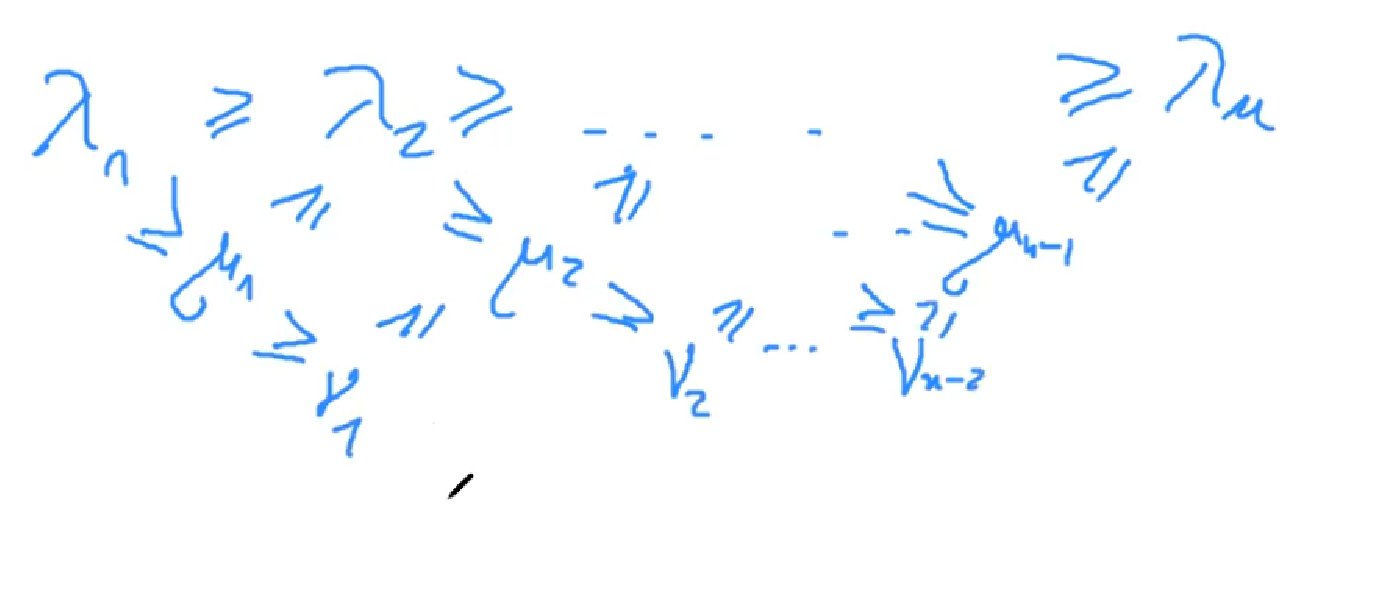
\includegraphics[scale=0.5]{eigen_prop.eps}

	Z obrazku
	\[ \lambda_i \geq k_i \lambda_{i + k} i = 1,2,..., n-k  \]

\end{proof}

\begin{theorem}[Nezav mnozina a vl cisla]
	Necht G je graf o n vrcholech s vl cisly $\lambda_1 \geq \lambda_2 \geq ... \geq \lambda_n$. Pak
	\[ \alpha(G) \leq \min\{|\{i : \lambda_i \leq 0\}|, |\{i : \lambda_i \geq 0\}|\} \]
\end{theorem}
\begin{proof}
	Necht $W \subseteq V(G)$ je nezav mnozina velkosti $\alpha$. Matice sousednosti teto mnoziny je nulova $\alpha \times \alpha$.
	Taky je to hlavne podmatice $A_G$. Proto jeji vl. cisle (nuly) propletaji vl cisla G. Z toho
	\[ \lambda_{\alpha} \geq 0 \geq \lambda_{n - \alpha + 1} \]
\end{proof}
